\section{Two-level systems at millikelvin}\label{sec:16.8}

One gram of fused silica cooled to \SI{10}{mK} is still giving off \SI{46}{pW} an hour later, and the power falls only as $1/t$ (\cref{we:16-heat}). For a detector held at \SI{10}{mK} this is a heat load that lasts for weeks. The heat comes from the tunneling two-level systems of \cref{sec:16.7}. Each was in equilibrium at a few kelvin, and each gives up its excess energy when it next relaxes, which for a defect behind a thick barrier takes hours or years. The same relaxation rates decide how fast a two-level system in a sensor film absorbs the energy of a phonon and returns it, and they are the kinetics behind the delayed signals of \cref{sec:19.6}. The defect is the two-configuration system of \cref{eq:C.20-H}, treated in the spin--boson language of \cref{app:C.20}.

\subsection{Relaxation by one phonon}\label{sec:16.8-phonon}

A two-level system relaxes when it passes from the upper to the lower of its two eigenstates and gives the splitting to its surroundings. The environment couples to the configuration through $\tfrac12\sigma_z X$, with $X = \sum_k\lambda_k(d_k + d_k^\dagger)$ the bath coordinate of \cref{eq:C.20-H}. By \cref{eq:16.7-rot} only the off-diagonal element $\Delta_0/\Delta_{\mathrm{tl}}$ of $\sigma_z$ in the eigenbasis changes the state; the diagonal part shifts the splitting by the fluctuating bath and contributes only to the dephasing. By the golden rule of \cref{sec:2.1} the emission of a bath quantum of energy $\Delta_{\mathrm{tl}}$ has the rate $2\pi\sum_k(\Delta_0\lambda_k/2\Delta_{\mathrm{tl}})^2(n_{\mathrm{B}} + 1)\,\delta(\Delta_{\mathrm{tl}} - \omega_k)$, and absorption has the same rate with $n_{\mathrm{B}}$ in place of $n_{\mathrm{B}} + 1$. A population difference relaxes at the sum of the two, which carries $2n_{\mathrm{B}} + 1 = \coth(\Delta_{\mathrm{tl}}/2T)$:
\begin{equation}
  \varGamma_1 = \frac12\Bigl(\frac{\Delta_0}{\Delta_{\mathrm{tl}}}\Bigr)^2 J_{\mathrm{s}}(\Delta_{\mathrm{tl}})\,\coth\frac{\Delta_{\mathrm{tl}}}{2T} .
  \label{eq:16.8-golden}
\end{equation}
The bath enters only through its spectral density $J_{\mathrm{s}}(\omega) = \pi\sum_k\lambda_k^2\delta(\omega - \omega_k)$ of \cref{eq:C.20-J} at the splitting. The rate is first order in $J_{\mathrm{s}}$, and it holds as long as $\varGamma_1 \ll \Delta_{\mathrm{tl}}$, so that the eigenstates are defined; its upward and downward parts obey detailed balance (\cref{sec:2.5}).

A long acoustic wave couples through the strain term of \cref{eq:16.7-H1}, and the deformation potential depends on the orientation of the defect relative to the wave. As in \cref{sec:16.7}, $\gamma_{\mathrm{l}}^2$ and $\gamma_{\mathrm{t}}^2$ are its mean squares over orientations for a longitudinal wave and for each transverse wave; acoustic experiments on glasses give about \SI{1}{eV}~\cite[Sect.~IV\,A]{muller2019towards}. Summing the strain of every phonon mode of \cref{sec:5.3} at the defect (\cref{app:D.42}) gives
\begin{equation}
  J_{\mathrm{s}}^{\mathrm{ph}}(\omega) = \frac{\omega^3}{\pi\rho_T}\Bigl(\frac{\gamma_{\mathrm{l}}^2}{c_{\mathrm{LA}}^5} + \frac{2\gamma_{\mathrm{t}}^2}{c_{\mathrm{TA}}^5}\Bigr) = 2K_{\mathrm{ph}}\,\omega^3 ,
  \label{eq:16.8-Jph}
\end{equation}
with $c_{\mathrm{LA}}$ and $c_{\mathrm{TA}}$ the sound speeds and $K_{\mathrm{ph}}$ the constant of \cref{eq:16.7-tau1}. The bath is superohmic (\cref{app:C.20}): the strain of one phonon grows as $\omega^{1/2}$ and the number of modes as $\omega^2$. With \cref{eq:16.8-golden} it gives the one-phonon rate $\varGamma_1^{\mathrm{ph}} = K_{\mathrm{ph}}\Delta_{\mathrm{tl}}^3(\Delta_0/\Delta_{\mathrm{tl}})^2\coth(\Delta_{\mathrm{tl}}/2T)$ of \cref{eq:16.7-tau1}. This is Jäckle's rate, in the form of Meißner et al.~\cite[Eq.~(7)]{meissner2021acoustic} and of Sahling et al.~\cite[Eqs.~(4), (5)]{sahling2010anomalous}. The fifth power of the sound speed makes the transverse waves dominate. At equal deformation potentials they carry $2(c_{\mathrm{LA}}/c_{\mathrm{TA}})^5 = 16.6$ times the longitudinal rate in vitreous silica, with the sound speeds of \cref{sec:16.7}, and 65 times in aluminum. A thermal defect, with $\Delta_{\mathrm{tl}} \approx T$ and fixed $\Delta_0/\Delta_{\mathrm{tl}}$, relaxes at a rate $\propto T^3$, and since $\Delta_0 \propto \ee^{-\lambda_{\mathrm{tun}}}$ the rate spans many decades across the broad distribution of tunneling exponents $\lambda_{\mathrm{tun}}$. A defect of \SI{5}{GHz}, $\Delta_{\mathrm{tl}} = \SI{20.7}{\micro eV}$, with $\Delta_0 = 0.3\,\Delta_{\mathrm{tl}}$ and $\gamma_{\mathrm{l}} = \gamma_{\mathrm{t}} = \SI{1}{eV}$, relaxes in aluminum at $2.1\times10^5\,\si{s^{-1}}$ below about \SI{50}{mK} ($2.5\times10^5\,\si{s^{-1}}$ at \SI{0.1}{K}; \cref{fig:16-tlsrates}).

\subsection{Relaxation by conduction electrons}\label{sec:16.8-electron}

In a metal the defect has a second bath. When it tunnels, the potential that scatters the conduction electrons changes, and the Fermi sea must rearrange. The excitations of the sea are electron--hole pairs, and near the Fermi level their number at energy $\omega$ grows as $\omega$ while the matrix elements stay constant, so the bath is ohmic, \cref{eq:C.20-ohmic}, with $J_{\mathrm{s}}^{\mathrm{el}}(\omega) = 2\pi\alpha_{\mathrm{ohm}}\omega$ for $\omega$ far below the cutoff. In \cref{eq:16.8-golden} it gives
\begin{equation}
  \varGamma_1^{\mathrm{el}} = \pi\alpha_{\mathrm{ohm}}\Bigl(\frac{\Delta_0}{\Delta_{\mathrm{tl}}}\Bigr)^2\Delta_{\mathrm{tl}}\,\coth\frac{\Delta_{\mathrm{tl}}}{2T} ,
  \label{eq:16.8-black}
\end{equation}
the rate of Black and coworkers, as quoted by Meißner et al.~\cite[Eq.~(8)]{meissner2021acoustic} with their coupling $W_{\mathrm{el}}^2 = 4\alpha_{\mathrm{ohm}}$. For a thermal defect it grows only linearly in $T$, against $T^3$ for one phonon, and below a kelvin the electrons win by orders of magnitude. For the \SI{5}{GHz} defect above in normal aluminum, $\varGamma_1^{\mathrm{el}} = 2.5\times10^9\,\si{s^{-1}}$ at \SI{10}{mK} with $\alpha_{\mathrm{ohm}} = 0.28$, against $2.1\times10^5\,\si{s^{-1}}$ for one phonon.

The coupling $\alpha_{\mathrm{ohm}}$ is fixed by how differently the two configurations scatter electrons at the Fermi level. Let the two configurations act on the electrons as contact potentials $\pm V_{\mathrm{d}}$ over a volume $\Omega$. To second order in $V_{\mathrm{d}}$ the electron--hole pairs then form a Gaussian bath, and their spectral density gives (\cref{app:D.42})
\begin{equation}
  \alpha_{\mathrm{ohm}} = 4K_{\mathrm{b}} , \qquad K_{\mathrm{b}} = (\mathcal{N}_{\mathrm{F}}V_{\mathrm{d}}\Omega)^2 ,
  \label{eq:16.8-born}
\end{equation}
with $\mathcal{N}_{\mathrm{F}}$ the density of states per spin. This is the coupling $K$ of Maillet et al.~\cite[Eq.~(4)]{maillet2023nanomechanical}, whose rate $4\pi K\Delta_0^2\coth(\Delta_{\mathrm{tl}}/2T)/\Delta_{\mathrm{tl}}$ is \cref{eq:16.8-black}; their fits to the damping of aluminum-coated nanomechanical resonators give $K = 0.07$ and 0.11, that is $\alpha_{\mathrm{ohm}} = 0.28$ and 0.44, with a single-spin density of states. Beyond the Born limit the coupling is \cref{eq:E.10-ohm}, a sum over the squared differences $\tilde\delta_\nu$ of the scattering phases of the two configurations. For one contact channel per spin the phases are $\mp\arctan(\pi\mathcal{N}_{\mathrm{F}}V_{\mathrm{d}}\Omega)$, and $\alpha_{\mathrm{ohm}} = (4/\pi^2)\arctan^2(\pi K_{\mathrm{b}}^{1/2})$, which saturates at one when the phase difference reaches $\pi$. The Born value is \SI{10}{\percent} high already at $K_{\mathrm{b}} = 0.017$ (\cref{lim:16.8a}). At the fitted $K_{\mathrm{b}} = 0.07$ the same contact potential gives $\alpha_{\mathrm{ohm}} = 0.19$, not 0.28; read the other way, the measured rate needs a contact potential \SI{32}{\percent} stronger than the Born estimate.

A first-principles $\alpha_{\mathrm{ohm}}$ needs the two relaxed configurations of the defect, from a nudged-elastic-band search (\cref{app:E.11}). It also needs the scattering matrices of the conduction electrons at the Fermi level in both, from an impurity Green's function or from the overlap of the two many-electron ground states as a function of the supercell size (\cref{app:E.10}). \Cref{app:E.22} specifies the calculation for a crowdion in tungsten, hydrogen in niobium and two-level systems in aluminum, its oxide and amorphous WSi, with the Born limit and the resonator fits as acceptance tests. No such calculation exists yet, and the fitted values are the only numbers in hand.

Below $T_c$ the electrons pair. A defect with $\Delta_{\mathrm{tl}} < 2\Delta_{\mathrm{BCS}}$ cannot break a pair, and it can only scatter the thermal quasiparticles of \cref{sec:7.2}, whose number falls as $\ee^{-\Delta_{\mathrm{BCS}}/T}$. A static change of potential is even under time reversal, so the quasiparticle matrix elements carry the case-I coherence factor of the electron density, and the golden-rule integral over the quasiparticle energies is done in \cref{app:D.42}. For $\Delta_{\mathrm{tl}}$ and $T$ both small compared with $\Delta_{\mathrm{BCS}}$ it gives
\begin{equation}
  \frac{\varGamma_1^{\mathrm{s}}}{\varGamma_1^{\mathrm{el}}} = \frac{2}{1 + \ee^{\Delta_{\mathrm{BCS}}/T}}\;\sinh\frac{\Delta_{\mathrm{tl}}}{2T}\;K_1\Bigl(\frac{\Delta_{\mathrm{tl}}}{2T}\Bigr) ,
  \label{eq:16.8-sc}
\end{equation}
with $K_1(u) = \int_0^\infty\dd\theta\,\ee^{-u\cosh\theta}\cosh\theta$ the modified Bessel function. The last two factors tend to one as $\Delta_{\mathrm{tl}}/T \to 0$, and the remaining factor $2/(1 + \ee^{\Delta_{\mathrm{BCS}}/T})$, twice the occupation of the gap edge, is the superconducting form of Meißner et al.~\cite[Eq.~(9)]{meissner2021acoustic}, which they state for $\Delta_{\mathrm{tl}} \ll \Delta_{\mathrm{BCS}}$. The same factor gives the ratio of ultrasonic attenuation in the superconducting and normal states, and for the same reason: both probes scatter quasiparticles through the density. The Bessel factor arises because $\Delta_{\mathrm{tl}}$ is not small compared with $T$. Normal electrons accept $\Delta_{\mathrm{tl}}$ from the whole Fermi sea, while quasiparticles crowd at the gap edge and the energy must be taken up within their thermal spread. The factor is 0.86 for a thermal defect with $\Delta_{\mathrm{tl}} = T$ and 0.71 at $\Delta_{\mathrm{tl}} = 2T$, and the form of the source holds within \SI{10}{\percent} only for $\Delta_{\mathrm{tl}} \le 0.7\,T$ (\cref{lim:16.8a}).

\Cref{fig:16-tlsrates} puts the three rates together for one defect in aluminum. In the normal state the electrons dominate at every temperature. Below $T_c$ the suppression is so strong that one phonon takes over below \SI{0.21}{K}, about $T_c/6$, and at \SI{50}{mK} the electron rate is $2\times10^{-9}\,\si{s^{-1}}$. A superconducting film at the base temperature of a dilution refrigerator thus leaves its two-level systems coupled to phonons alone, as an insulator would.

\begin{figure}[tbp]
  \centering
  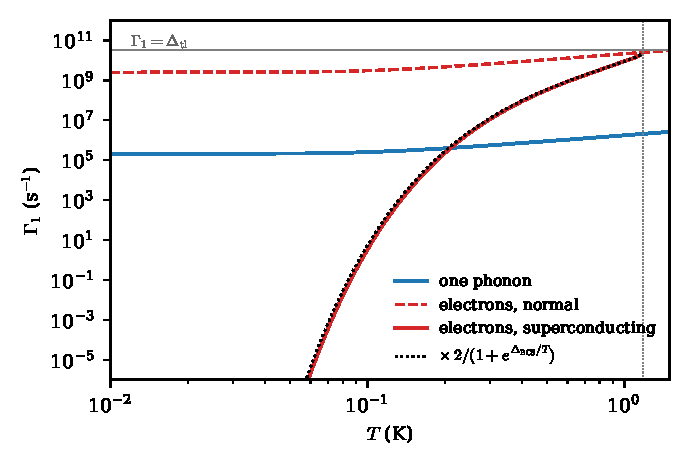
\includegraphics[width=0.7\linewidth]{figures/ch16/fig16_8.pdf}
  \caption{Relaxation rates of one two-level system in aluminum against temperature, for $\Delta_{\mathrm{tl}} = \SI{20.7}{\micro eV}$ (\SI{5}{GHz}) and $\Delta_0 = 0.3\,\Delta_{\mathrm{tl}}$. Blue: one phonon, \cref{eq:16.7-tau1}, with the model deformation potentials $\gamma_{\mathrm{l}} = \gamma_{\mathrm{t}} = \SI{1}{eV}$ and the isotropic sound speeds $c_{\mathrm{LA}} = \SI{6.63}{km.s^{-1}}$, $c_{\mathrm{TA}} = \SI{3.30}{km.s^{-1}}$ and density \SI{2.70}{g.cm^{-3}} of aluminum (\cref{sec:20.3}). Red dashed: conduction electrons in the normal state, \cref{eq:16.8-black}, with $\alpha_{\mathrm{ohm}} = 0.28$, continued below $T_c = \SI{1.18}{K}$ (vertical line) as for a film held normal. Red solid: the superconducting state, from the quasiparticle integral of \cref{app:D.42} with the weak-coupling gap $\Delta_{\mathrm{BCS}}(T)$; black dotted: the normal rate times $2/(1 + \ee^{\Delta_{\mathrm{BCS}}/T})$. The gray line marks $\varGamma_1 = \Delta_{\mathrm{tl}}$, which the normal-state rate reaches at \SI{1.5}{K}, where the golden rule fails.}
  \label{fig:16-tlsrates}
\end{figure}

\begin{limitbox}[Two-level relaxation by phonons and electrons][lim:16.8a]
The published rates are Jäckle's one-phonon rate and Black's electron rate, \cref{eq:16.7-tau1,eq:16.8-black}, with the superconducting factor $2/(1 + \ee^{\Delta_{\mathrm{BCS}}/T})$~\cite[Eqs.~(7)--(9)]{meissner2021acoustic}, and the Born-limit coupling $\alpha_{\mathrm{ohm}} = 4K_{\mathrm{b}}$~\cite[Eq.~(4)]{maillet2023nanomechanical}.
\par\smallskip
{\centering
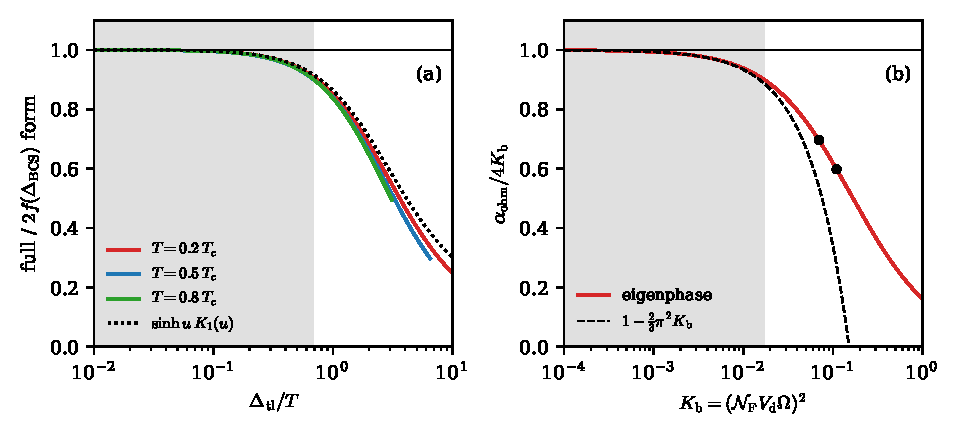
\includegraphics[width=\linewidth]{figures/ch16/limit16_8a.pdf}
\captionof{figure}{(a) Electron relaxation rate of a two-level system in superconducting aluminum, from the quasiparticle integral with the case-I coherence factor and the weak-coupling gap ($T_c = \SI{1.18}{K}$), divided by the normal rate times $2/(1 + \ee^{\Delta_{\mathrm{BCS}}/T})$, against $\Delta_{\mathrm{tl}}/T$ at $T = 0.2$, 0.5 and $0.8\,T_c$; each curve ends at $\Delta_{\mathrm{tl}} = 2\Delta_{\mathrm{BCS}}(T)$. Dotted: the closed form $\sinh u\,K_1(u)$, $u = \Delta_{\mathrm{tl}}/2T$, of \cref{eq:16.8-sc}. Gray: within \SI{10}{\percent} of one, $\Delta_{\mathrm{tl}} \le 0.69$--$0.73\,T$. (b) Ohmic coupling from the scattering phases of one contact channel per spin, $\alpha_{\mathrm{ohm}} = (4/\pi^2)\arctan^2(\pi K_{\mathrm{b}}^{1/2})$, divided by the Born value $4K_{\mathrm{b}}$, against $K_{\mathrm{b}}$. Dashed: the leading correction $1 - \tfrac23\pi^2K_{\mathrm{b}}$. Dots: the resonator fits $K_{\mathrm{b}} = 0.07$ and 0.11. Gray: within \SI{10}{\percent}, $K_{\mathrm{b}} \le 0.017$.}\label{fig:16-limit-tlsrel}
\par}
\smallskip
For $\Delta_{\mathrm{tl}} \gtrsim T$ the quasiparticles cannot take up the splitting as freely as normal electrons, and for $K_{\mathrm{b}} \gtrsim 0.02$ the phase shift of a single channel is no longer small, so that the Born coupling overstates $\alpha_{\mathrm{ohm}}$.
\end{limitbox}

\subsection{The ohmic scaling limit}\label{sec:16.8-ohmic}

The fitted couplings are not small, and \cref{fig:16-tlsrates} shows the consequence: the normal-state rate of \cref{eq:16.8-black} reaches the splitting itself at \SI{1.5}{K}, and for a symmetric defect, $\Delta_0 = \Delta_{\mathrm{tl}}$, it is at least $0.88\,\Delta_{\mathrm{tl}}$ at every temperature, since $\varGamma_1^{\mathrm{el}}/\Delta_{\mathrm{tl}} = \pi\alpha_{\mathrm{ohm}}\coth(\Delta_{\mathrm{tl}}/2T)$ with $\alpha_{\mathrm{ohm}} = 0.28$. A defect damped at a rate comparable to its splitting has no eigenstates to relax between. The electrons then dephase the two configurations faster than the defect tunnels, and the defect hops between $|\mathrm{L}\rangle$ and $|\mathrm{R}\rangle$ at the incoherent rate of \cref{eq:C.20-rate}, second order in $\Delta_0$ and exact in $\alpha_{\mathrm{ohm}}$. \Cref{app:C.20} evaluates it for the ohmic bath, \cref{eq:C.20-ohmrate}, and shows that for $\Delta_0, T \ll \omega_{\mathrm{cut}}$ the cutoff enters only through the renormalized tunneling amplitude $\Delta_{\mathrm{r}}$ of \cref{eq:C.20-Dr}. For a symmetric defect the relaxation rate $\varGamma_{\mathrm{LR}} + \varGamma_{\mathrm{RL}}$ is then
\begin{equation}
  \varGamma_{\mathrm{LR}} + \varGamma_{\mathrm{RL}} = \frac{\Gamma(1 + \alpha_{\mathrm{ohm}})}{\Gamma(1 - \alpha_{\mathrm{ohm}})}\,\frac{\Delta_{\mathrm{r}}^{2(1 - \alpha_{\mathrm{ohm}})}}{\alpha_{\mathrm{ohm}}}\,(2\pi T)^{2\alpha_{\mathrm{ohm}} - 1} ,
  \qquad \Delta_{\mathrm{r}} \ll T \ll \omega_{\mathrm{cut}} ,
  \label{eq:16.8-scaling}
\end{equation}
with $\Gamma(z)$ Euler's gamma function; the form follows from \cref{eq:C.20-ohmrate} at $\Delta_{\mathrm{as}} = 0$ with the duplication and reflection formulas of $\Gamma$. The rate depends on $\Delta_0$ and $\omega_{\mathrm{cut}}$ only through $\Delta_{\mathrm{r}}$, which is what makes it a scaling limit. It grows as the temperature falls whenever $\alpha_{\mathrm{ohm}} < \tfrac12$, the anti-Arrhenius law: at $\alpha_{\mathrm{ohm}} = 0.28$ it scales as $T^{-0.44}$, and as $\alpha_{\mathrm{ohm}} \to 0$ as $1/T$. A thermally activated rate would do the opposite. \Cref{app:C.20} traces the growth to the slower dephasing by the electrons at low temperature, over the time $1/T$, which wins against the shrinking dressed amplitude.

Qureshi obtained the same dynamics from the bosonized electron gas~\cite{qureshi1995dynamics}. Without electron-assisted tunneling his Laplace-transformed correlation function of $\sigma_z$~\cite[Eqs.~(8), (9)]{qureshi1995dynamics} is the noninteracting-blip result of \cref{app:C.20}, and his coupling $K$ is $\alpha_{\mathrm{ohm}}$ in the normalization of \cref{eq:C.20-ohmic}, not $K_{\mathrm{b}}$. For a symmetric defect and $\alpha_{\mathrm{ohm}} \ll 1$ he reduces it to~\cite[Eq.~(10)]{qureshi1995dynamics}
\begin{equation}
  \begin{gathered}
  \hat C(z) \simeq \frac{1}{z + \tilde\Delta_0^2/(z + \gamma_0)} , \qquad \gamma_0 = 2\pi\alpha_{\mathrm{ohm}}T , \\
  \tilde\Delta_0^2 = \Gamma(1 - 2\alpha_{\mathrm{ohm}})\cos(\pi\alpha_{\mathrm{ohm}})\,\Delta_0^2\Bigl(\frac{2\pi T}{\omega_{\mathrm{cut}}}\Bigr)^{2\alpha_{\mathrm{ohm}}} .
  \end{gathered}
  \label{eq:16.8-qureshi}
\end{equation}
Its poles describe both regimes of this section. For $\tilde\Delta_0 > \gamma_0/2$ the defect oscillates at a frequency near $\tilde\Delta_0$ and its $\sigma_z$ correlation decays at $\gamma_0/2 = \pi\alpha_{\mathrm{ohm}}T$. For a symmetric defect with $T \gg \Delta_{\mathrm{tl}}$ this is half of \cref{eq:16.8-black}, the decay of an off-diagonal quantity at $\varGamma_1/2$, so Black's rate is the weakly damped side of \cref{eq:16.8-qureshi}. For $\tilde\Delta_0 < \gamma_0/2$ the motion is overdamped and the slow pole gives the relaxation rate $\tilde\Delta_0^2/\gamma_0$. By \cref{eq:C.20-Dr}, $\tilde\Delta_0^2 = \Delta_{\mathrm{r}}^{2(1 - \alpha_{\mathrm{ohm}})}(2\pi T)^{2\alpha_{\mathrm{ohm}}}$, and $\tilde\Delta_0^2/\gamma_0$ is \cref{eq:16.8-scaling} without the factor $\Gamma(1 + \alpha_{\mathrm{ohm}})/\Gamma(1 - \alpha_{\mathrm{ohm}}) = 1 - 2\gamma_{\mathrm{E}}\alpha_{\mathrm{ohm}} + O(\alpha_{\mathrm{ohm}}^2)$, which is \SI{10}{\percent} below one at $\alpha_{\mathrm{ohm}} = 0.091$ and 0.71 at the fitted 0.28 (\cref{lim:16.8b}). The boundary $\tilde\Delta_0 = \gamma_0/2$ is a temperature,
\begin{equation}
  T_{\mathrm{coh}} = \frac{\Delta_{\mathrm{r}}}{2\pi}\Bigl(\frac{2}{\alpha_{\mathrm{ohm}}}\Bigr)^{1/(1 - \alpha_{\mathrm{ohm}})} ,
  \label{eq:16.8-Tcoh}
\end{equation}
below which a symmetric defect tunnels coherently, with weak damping, and above which it hops. For $\alpha_{\mathrm{ohm}} \ll 1$ it is $\Delta_{\mathrm{r}}/\pi\alpha_{\mathrm{ohm}}$, the temperature at which $\pi\alpha_{\mathrm{ohm}}T$ reaches the splitting; at $\alpha_{\mathrm{ohm}} = 0.28$ the small-coupling form of \cref{eq:16.8-qureshi} puts it at $2.4\,\Delta_{\mathrm{r}}$, where the scaling form \cref{eq:16.8-scaling} is itself at the edge of its range. An asymmetric defect, $\Delta_{\mathrm{as}} \gg \Delta_0$, is weakly damped as long as \cref{eq:16.8-black} stays below $\Delta_{\mathrm{tl}}$, and most defects of a glass are of this kind (\cref{sec:16.7}); the scaling limit concerns the nearly symmetric ones and light interstitials in metals.

\begin{limitbox}[The ohmic scaling limit][lim:16.8b]
The published relaxation rate of a symmetric tunneling defect in a metal is $\tilde\Delta_0^2/\gamma_0$, from the slow pole of \cref{eq:16.8-qureshi}, for $\alpha_{\mathrm{ohm}} \ll 1$~\cite[Eqs.~(8)--(10)]{qureshi1995dynamics}.
\par\smallskip
{\centering
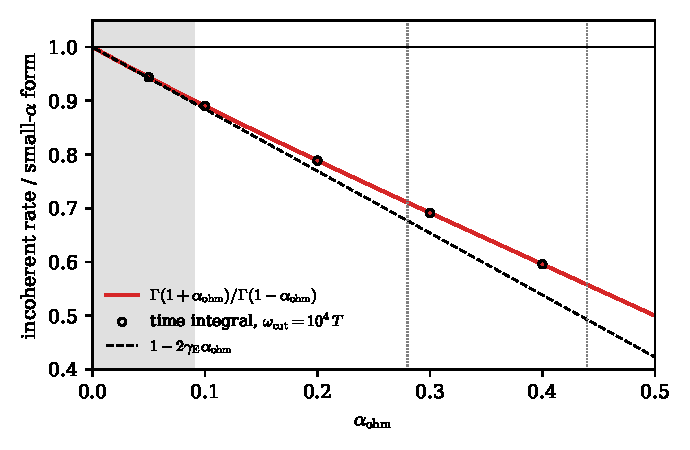
\includegraphics[width=0.75\linewidth]{figures/ch16/limit16_8b.pdf}
\captionof{figure}{Incoherent relaxation rate of a symmetric defect in an ohmic bath, \cref{eq:C.20-rate,eq:16.8-scaling}, divided by the small-coupling form $\tilde\Delta_0^2/\gamma_0$, against $\alpha_{\mathrm{ohm}}$. Red: the scaling limit $\Gamma(1 + \alpha_{\mathrm{ohm}})/\Gamma(1 - \alpha_{\mathrm{ohm}})$. Open circles: the time integral of \cref{eq:C.20-rate} done numerically with the full ohmic correlation exponent at $\omega_{\mathrm{cut}} = 10^4\,T$. Dashed: the leading correction $1 - 2\gamma_{\mathrm{E}}\alpha_{\mathrm{ohm}}$. Dotted lines: the Born values $\alpha_{\mathrm{ohm}} = 0.28$ and 0.44 of the aluminum resonator fits. Gray: within \SI{10}{\percent}, $\alpha_{\mathrm{ohm}} \le 0.091$.}\label{fig:16-limit-ohmic}
\par}
\smallskip
Outside the gray band the small-coupling form overstates the rate, by $1/0.71$ at $\alpha_{\mathrm{ohm}} = 0.28$, and both forms fail below $T \sim \Delta_{\mathrm{r}}$, where the defect tunnels coherently.
\end{limitbox}

\subsection{Thermally activated hopping and tunneling}\label{sec:16.8-hop}

A defect whose barrier $V_{\mathrm{b}}$ of \cref{sec:16.7} is large compared with $T$ can still cross it classically, at the rate $\varGamma = \varGamma_0\ee^{-V_{\mathrm{b}}/T}$ of harmonic transition-state theory (\cref{app:E.11}), with $\varGamma_0$ the attempt rate. In one dimension $\varGamma_0 = \omega_{\mathrm{w}}/2\pi$, with $\omega_{\mathrm{w}}$ the frequency of the well, and in many dimensions $\varGamma_0$ is Vineyard's ratio of the products of normal-mode frequencies at the minimum and at the saddle. This is the transition-state rate of Lawrence~\cite[Eq.~(1)]{lawrence2024semiclassical} with a classical, harmonic reactant partition function and transmission coefficient $\kappa = 1$. Tunneling through the top of the barrier raises the rate. For a barrier that is an inverted parabola of frequency $\omega^\ddagger$ the correction is exact,
\begin{equation}
  \kappa_{\mathrm{PB}} = \frac{\omega^\ddagger/2T}{\sin(\omega^\ddagger/2T)} = 1 + \frac{1}{24}\Bigl(\frac{\omega^\ddagger}{T}\Bigr)^2 + \frac{7}{5760}\Bigl(\frac{\omega^\ddagger}{T}\Bigr)^4 + \dots ,
  \label{eq:16.8-kappa}
\end{equation}
and its first two terms are Wigner's correction $\kappa_{\mathrm{W}}$~\cite[Eqs.~(2), (3)]{lawrence2024semiclassical}. The parabolic correction diverges at the crossover temperature
\begin{equation}
  T_\times = \frac{\omega^\ddagger}{2\pi} ,
  \label{eq:16.8-Tx}
\end{equation}
below which the particle no longer crosses near the top. It tunnels through the barrier at the energy that maximizes the product of the thermal weight and the transmission, along the instanton, the periodic path in imaginary time of period $1/T$, whose action $S_{\mathrm{inst}}$ replaces $V_{\mathrm{b}}/T$ in the exponent~\cite[Eq.~(4)]{lawrence2024semiclassical}. As $T \to 0$ the instanton becomes the tunneling path between the two minima, its action becomes twice the tunneling exponent $\lambda_{\mathrm{tun}}$ of \cref{sec:16.7}, and the hopping turns into the tunneling between $|\mathrm{L}\rangle$ and $|\mathrm{R}\rangle$ with amplitude $\Delta_0 \propto \ee^{-\lambda_{\mathrm{tun}}}$ that the previous sections assumed. For an atom with $\omega^\ddagger = \SI{10}{meV}$, $T_\times = \SI{18.5}{K}$, so at millikelvin temperatures every defect motion is tunneling, and a defect whose $\lambda_{\mathrm{tun}}$ is too large for it to tunnel within the time of an experiment is frozen. With an attempt rate of \SI{e13}{s^{-1}} and a year of observation, the bound is $\lambda_{\mathrm{tun}} \le 23.6$ when no energy-gap suppression adds to the exponent (\cref{app:E.22}).

\Cref{lim:16.8c} tests these forms on a barrier whose quantum rate is known exactly, the symmetric Eckart barrier $V(x) = V_{\mathrm{b}}\,\mathrm{sech}^2(x/L)$ with the hydrogen-atom parameters of Lawrence, $V_{\mathrm{b}} = 6\omega^\ddagger/\pi$. The exact rate exceeds the classical one by a factor 6.2 at $T_\times$ and 2.2 at $1.5\,T_\times$, so tunneling matters well above the crossover. Wigner's correction holds within \SI{10}{\percent} above $2.1\,T_\times$ and the parabolic form above $1.5\,T_\times$, while the instanton rate stays about \SI{18}{\percent} low between $0.25$ and $0.5\,T_\times$, an error that the higher terms of its asymptotic expansion in $\hbar$ would reduce~\cite[Sect.~III\,A]{lawrence2024semiclassical}.

Activation also fixes which defects of a glass contribute to its heat release. On cooling, defects with large barriers stay in equilibrium by activation until the activated rate falls below the rate at which the cooling changes $V_{\mathrm{b}}/T$, which is $V_{\mathrm{b}}|\dot T|/T^2$. Equating the two gives the freezing temperature
\begin{equation}
  T_{\mathrm{frz}} = \frac{V_{\mathrm{b}}}{\ln\bigl(\varGamma_0T_{\mathrm{frz}}^2/V_{\mathrm{b}}|\dot T|\bigr)} ,
  \label{eq:16.8-Tfrz}
\end{equation}
the form of Sahling et al.~\cite[Eq.~(8)]{sahling2010anomalous} with their $\tau_0 = 1/\varGamma_0$. Below $T_{\mathrm{frz}}$ the populations of these defects stop following the temperature, and the excess they keep is released later by tunneling.

\begin{limitbox}[Hopping and tunneling through one barrier][lim:16.8c]
The published rates are transition-state theory with Wigner's or the parabolic-barrier transmission, \cref{eq:16.8-kappa}, above the crossover temperature \cref{eq:16.8-Tx}, and the instanton rate below it~\cite[Eqs.~(1)--(4)]{lawrence2024semiclassical}.
\par\smallskip
{\centering
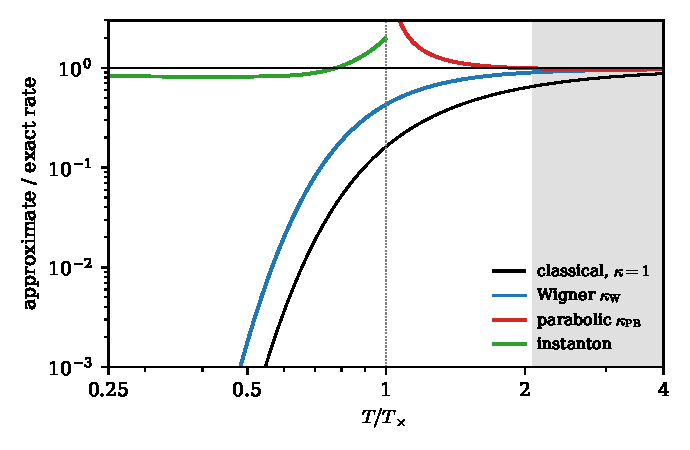
\includegraphics[width=0.75\linewidth]{figures/ch16/limit16_8c.pdf}
\captionof{figure}{Approximate thermal rates through a symmetric Eckart barrier divided by the exact quantum rate, against $T/T_\times$, for the hydrogen-atom parameters of Lawrence ($V_{\mathrm{b}} = \SI{248}{meV}$, $\omega^\ddagger = \SI{130}{meV}$, $T_\times = \SI{240}{K}$). Black: classical transition-state theory. Blue: with Wigner's correction. Red: with the parabolic-barrier correction, divergent at $T_\times$ (dotted line). Green: the instanton rate, for $T < T_\times$. The exact rate integrates the exact transmission probability of the Eckart barrier over the Boltzmann factor. Gray: Wigner's form within \SI{10}{\percent}, $T \ge 2.1\,T_\times$.}\label{fig:16-limit-hop}
\par}
\smallskip
Near $T_\times$ the expansion in $\omega^\ddagger/T$ diverges and the instanton is not yet formed, so neither form holds there, and below $T_\times$ the transition-state forms underestimate the rate by orders of magnitude.
\end{limitbox}

\subsection{Heat release of a cooled glass}\label{sec:16.8-heat}

A glass held at $T_{\mathrm{hi}}$ and cooled quickly to $T_{\mathrm{lo}}$ keeps its slow defects in the populations of $T_{\mathrm{hi}}$. A defect of splitting $\Delta_{\mathrm{tl}}$ has the mean energy $-\tfrac12\Delta_{\mathrm{tl}}\tanh(\Delta_{\mathrm{tl}}/2T)$ in equilibrium, so it holds the excess $\tfrac12\Delta_{\mathrm{tl}}[\tanh(\Delta_{\mathrm{tl}}/2T_{\mathrm{lo}}) - \tanh(\Delta_{\mathrm{tl}}/2T_{\mathrm{hi}})]$, which it gives to the phonons at its rate $\varGamma_1$ of \cref{eq:16.7-tau1}, evaluated at $T_{\mathrm{lo}}$. The defects are spread uniformly in the asymmetry $\Delta_{\mathrm{as}}$ and in the tunneling exponent $\lambda_{\mathrm{tun}}$, with density $\bar P$ (\cref{sec:16.7-stm})~\cite[Eq.~(1)]{sahling2010anomalous}. The slow defects have $\Delta_0 \ll \Delta_{\mathrm{as}}$, so $\Delta_{\mathrm{tl}} \simeq \Delta_{\mathrm{as}}$ is distributed uniformly too. Their excess energy, summed over $\Delta_{\mathrm{tl}}$, is
\begin{equation*}
  \int_0^\infty\dd\Delta_{\mathrm{tl}}\,\frac{\Delta_{\mathrm{tl}}}{2}\Bigl[\tanh\frac{\Delta_{\mathrm{tl}}}{2T_{\mathrm{lo}}} - \tanh\frac{\Delta_{\mathrm{tl}}}{2T_{\mathrm{hi}}}\Bigr] = \frac{\pi^2}{12}\bigl(T_{\mathrm{hi}}^2 - T_{\mathrm{lo}}^2\bigr) ,
\end{equation*}
since $1 - \tanh(x/2T) = 2/(\ee^{x/T} + 1)$ and $\int_0^\infty\dd x\,x/(\ee^{x/T} + 1) = \pi^2T^2/12$. The rate depends on the tunneling exponent through $\Delta_0^2 \propto \ee^{-2\lambda_{\mathrm{tun}}}$, so at fixed $\Delta_{\mathrm{tl}}$ a uniform density in $\lambda_{\mathrm{tun}}$ is a uniform density $\tfrac12$ per unit $\ln\varGamma_1$. A defect relaxes at time $t$ with probability $\varGamma_1\ee^{-\varGamma_1t}\dd t$, and summing over $\lambda_{\mathrm{tun}}$ gives $\int\dd\lambda_{\mathrm{tun}}\,\varGamma_1\ee^{-\varGamma_1t} = \tfrac12\int\dd\varGamma_1\,\ee^{-\varGamma_1t} = 1/2t$ whenever the rates extend far on both sides of $1/t$. The power released by a volume $\Vol$ of glass is therefore
\begin{keyresult}[Heat release of a cooled glass]
\begin{equation}
  \dot Q_{\mathrm{TLS}}(t) = \frac{\pi^2}{24}\,\bar P\,\Vol\,\frac{T_{\mathrm{hi}}^2 - T_{\mathrm{lo}}^2}{t} , \qquad \varGamma_{\max}^{-1} \ll t \ll \varGamma_{\min}^{-1} ,
  \label{eq:16.8-heat}
\end{equation}
\end{keyresult}
with $\varGamma_{\max}$ and $\varGamma_{\min}$ the fastest and slowest one-phonon rates at $T_{\mathrm{lo}}$ of the defects with $\Delta_{\mathrm{tl}} \sim T_{\mathrm{hi}}$, which hold most of the excess. This is the law of Sahling et al.~\cite[Eq.~(6)]{sahling2010anomalous}. The $1/t$ comes from the uniform density in $\lambda_{\mathrm{tun}}$, and the prefactor depends neither on the deformation potentials nor on the sound speeds, which only shift the window in time. Since every decade of time draws on defects in a range of $\lambda_{\mathrm{tun}}$ of width $\tfrac12\ln10$, the heat released between $t_1$ and $t_2$ is the prefactor times $\ln(t_2/t_1)$, and the heat measured at a time $t$ comes from defects with $\varGamma_1 \approx 1/t$. If the glass starts above $T_{\mathrm{frz}}$ of \cref{eq:16.8-Tfrz}, the defects that release at time $t$ were last in equilibrium at $T_{\mathrm{frz}}$, and $T_{\mathrm{frz}}$ replaces $T_{\mathrm{hi}}$~\cite[Eq.~(7)]{sahling2010anomalous}; the release then no longer grows with the starting temperature.

\begin{limitbox}[Heat release of a cooled glass][lim:16.8d]
The published heat release after a quench from $T_{\mathrm{hi}}$ to $T_{\mathrm{lo}}$ is \cref{eq:16.8-heat}~\cite[Eqs.~(1), (6)--(8)]{sahling2010anomalous}.
\par\smallskip
{\centering
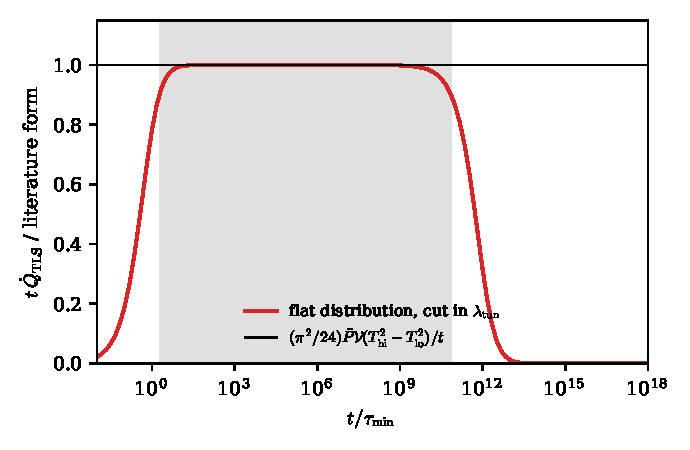
\includegraphics[width=0.75\linewidth]{figures/ch16/limit16_8d.pdf}
\captionof{figure}{Heat release of a model glass times $t$, divided by the prefactor of \cref{eq:16.8-heat}, against $t$ in units of $\tau_{\min}$, the relaxation time of the fastest defect at $\Delta_{\mathrm{tl}} = T_{\mathrm{hi}}$. Red: the uniform distribution cut at $\lambda_{\mathrm{min}} \le \lambda_{\mathrm{tun}} \le \lambda_{\mathrm{min}} + 14$, with the exact splitting $\Delta_{\mathrm{tl}} = (\Delta_{\mathrm{as}}^2 + \Delta_0^2)^{1/2}$, $\Delta_0 \le 0.1\,T_{\mathrm{lo}}$, the one-phonon rate \cref{eq:16.7-tau1} at $T_{\mathrm{lo}}$ and an instantaneous quench with $T_{\mathrm{lo}}/T_{\mathrm{hi}} = 1/480$ (\SI{10}{mK} after \SI{4.8}{K}). Gray: within \SI{10}{\percent} of one, $1.8\,\tau_{\min} \le t \le 7.1\times10^{10}\,\tau_{\min}$, 10.6 of the 12.2 decades that the cut spans.}\label{fig:16-limit-heat}
\par}
\smallskip
Outside the window the release falls below the $1/t$ law, at early times because the fastest defects have already relaxed and at late times because the distribution of tunneling exponents ends.
\end{limitbox}

Inside its window \cref{eq:16.8-heat} is exact for the uniform distribution: in \cref{lim:16.8d} it holds within $2\times10^{-4}$ from $10^2$ to $10^8\,\tau_{\min}$. The tests of the law are therefore tests of the distribution. Heat-release measurements on vitreous silica follow $1/t$ and $T_{\mathrm{hi}}^2 - T_{\mathrm{lo}}^2$, but they give a density $\bar P$ four times smaller than the specific heat measured over seconds, $2.0\times10^{44}$ against $8.0\times10^{44}\,\si{J^{-1}.m^{-3}}$~\cite[Table~1]{sahling2014anomalous}. Sahling et al.\ attribute the difference to defects whose barriers are lowered by local stresses frozen in on cooling. These relax within about \SI{100}{s}, before the heat-release measurement starts, and a small fraction of them, \SI{5}{\percent}, freezes at \SI{14.5}{K} instead of \SI{4.8}{K} and adds to the release after a quench from higher temperatures~\cite{sahling2014anomalous}. The specific-heat value, $1.28\times10^{20}\,\si{eV^{-1}.cm^{-3}}$, is close to the $1.2\times10^{20}\,\si{eV^{-1}.cm^{-3}}$ that the polarization-averaged acoustic tunneling strength implies for $\gamma_{\mathrm{l}} = \SI{1}{eV}$ ($0.88\times10^{20}$ with the longitudinal $C_{\mathrm{l}}$; \cref{sec:16.7}).

\begin{workedexample}{Heat release of one gram of fused silica at \SI{10}{mK}}\label{we:16-heat}
Take \SI{1}{g} of vitreous silica, $\Vol = \SI{0.455}{cm^3}$ at the density $\rho_T = \SI{2.2}{g.cm^{-3}}$ of \cref{sec:16.7}, cooled from room temperature to $T_{\mathrm{lo}} = \SI{10}{mK}$. The defects that release over hours to weeks freeze at $T_{\mathrm{frz}} = \SI{4.8}{K}$, and the heat-release density is $\bar P = 2.0\times10^{44}\,\si{J^{-1}.m^{-3}} = 3.20\times10^{19}\,\si{eV^{-1}.cm^{-3}}$~\cite[Table~1]{sahling2014anomalous}. With $T_{\mathrm{frz}}$ in place of $T_{\mathrm{hi}}$, and $T_{\mathrm{lo}}^2/T_{\mathrm{frz}}^2 = 4\times10^{-6}$ negligible, \cref{eq:16.8-heat} gives
\begin{equation*}
  \begin{split}
  t\,\dot Q_{\mathrm{TLS}} &= \frac{\pi^2}{24}\,k_{\mathrm{B}}^2\,\bar P\,\Vol\,T_{\mathrm{frz}}^2 \\
  &= 0.4112\times(\SI{1.381e-23}{J.K^{-1}})^2\times\SI{2.0e44}{J^{-1}.m^{-3}} \\
  &\qquad\times\SI{4.55e-7}{m^3}\times(\SI{4.8}{K})^2 \\
  &= \SI{1.64e-7}{J} .
  \end{split}
\end{equation*}
One hour after the cooling the sample releases $\SI{1.64e-7}{J}/\SI{3600}{s} = \SI{46}{pW}$, after a day \SI{1.9}{pW}, and after a week \SI{0.27}{pW}. Between the first hour and the end of the first week it gives off $\SI{1.64e-7}{J}\times\ln168 = \SI{0.84}{\micro J}$, or $5\times10^{12}\,\si{eV}$. With the specific-heat density the power would be four times larger. The fraction of defects that freezes at \SI{14.5}{K} is $0.05\times3 = 0.15$ of the normal density, with 3 the ratio of the stress-lowered defects to the normal density, $(8.0 - 2.0)/2.0$. By the square of its freezing temperature it adds another 1.4 times the normal release after a quench from above \SI{14.5}{K}, with the freezing temperatures of the table of Sahling et al. Their text quotes 5.5 and \SI{14.1}{K}, which give 0.99, and states that the anomalous part is roughly twice the normal one~\cite{sahling2014anomalous}. A hundred grams of fused silica near a detector at \SI{10}{mK} thus deposits \SI{4.6}{nW} an hour after cooling and \SI{0.19}{nW} a day later, a load and a source of delayed events that \cref{sec:19.6} takes up.
\end{workedexample}

\subsection{Interacting two-level systems}\label{sec:16.8-open}

Every result of this section treats the defects as independent, yet two defects interact through the strain fields each creates, with a coupling that falls as $1/r^3$. Its typical size relative to the spread of their splittings is the tunneling strength $C = \bar P\gamma_{\mathrm{l}}^2/\rho_Tc_{\mathrm{LA}}^2$, $2.6\times10^{-4}$ in vitreous silica (\cref{sec:16.7}). Thermal flips of neighbors shift the splitting of a given defect in time, which is spectral diffusion; it broadens single lines, and qubit spectroscopy sees it directly~\cite[Sect.~IV]{muller2019towards}. An ensemble whose spectrum is flat in $\Delta_{\mathrm{tl}}$ is unchanged by a normalized shift kernel away from the edges of the band. Spectral diffusion alone therefore leaves the ensemble responses of \cref{sec:16.7} intact, but it changes which defects relax at a given time and so the window of \cref{eq:16.8-heat}. The phonon emitted by one relaxing defect can trigger the relaxation of another. If each release triggers on average $b_{\mathrm{br}}$ more, a branching process, the mean size of a cascade of releases is $1/(1 - b_{\mathrm{br}})$, finite for $b_{\mathrm{br}} < 1$, and the distribution of the cascade size $N_{\mathrm{casc}}$ approaches $N_{\mathrm{casc}}^{-3/2}$ as $b_{\mathrm{br}} \to 1$. Such avalanches would turn the steady $1/t$ release into bursts. None of this is quantified for a real glass: $b_{\mathrm{br}}$ needs the density of barriers below the energy of the emitted phonons and the flux of ballistic phonons through the triggering volume, and no calculation or measurement of it exists. Whether the delayed events of a cooled detector are independent relaxations or avalanches of this kind is the open question that \cref{sec:19.6} inherits.
